% !TEX program = xelatex
% 题目：医学影像分割的基础模型方法：从 SAM 到 MedSAM 的提示策略与少样本适配研究
% 编译：xelatex -> bibtex -> xelatex -> xelatex（在 paper/ 目录内执行）
% 所有实验数字均取自 results/ 目录落盘文件（metrics.csv / dataset_stats.csv / summary.json）
\documentclass[zihao=-4,a4paper]{ctexart}

\usepackage[margin=2.6cm]{geometry}
\usepackage{amsmath,amssymb}
\usepackage{graphicx}
\usepackage{booktabs}
\usepackage{multirow}
\usepackage{float}
\usepackage{caption}
\usepackage{enumitem}
\usepackage{tikz}
\usetikzlibrary{arrows.meta,positioning,fit,calc}

\captionsetup{font=small,labelfont=bf}
\setlength{\parskip}{0.2ex}
% 带圈数字（U+2460--246F）交由中文字体渲染（Latin Modern 无该区字形）
\xeCJKDeclareCharClass{CJK}{"2460 -> "246F}

\title{\heiti 医学影像分割的基础模型方法：\\从 SAM 到 MedSAM 的提示策略与少样本适配研究}
\author{}
\date{}

\begin{document}

% ==================== 封面 ====================
\begin{titlepage}
\centering
\vspace*{3.5cm}
{\zihao{3}\heiti 医学影像分割的基础模型方法：\\[0.6em]从 SAM 到 MedSAM 的提示策略与少样本适配研究\par}
\vspace{3.5cm}
{\zihao{-3}
\renewcommand{\arraystretch}{1.7}
\begin{tabular}{rl}
姓\hspace{2em}名： & 王鸿希 \\
学\hspace{2em}院： & 计算机与大数据 \\
日\hspace{2em}期： & 2026 年 10 月 24 日 \\
\end{tabular}\par}
\vfill
\end{titlepage}

% ==================== 正文页码从 1 开始 ====================
\pagenumbering{arabic}
\setcounter{page}{1}

% ==================== 中文摘要 ====================
\begin{center}
{\zihao{4}\heiti 摘\quad 要}
\end{center}

医学图像分割长期依赖逐任务的大规模专家标注与专用模型训练，标注瓶颈严重制约新临床任务的落地速度。分割一切模型（SAM）及其医学变体 MedSAM 带来了``提示式分割''的基础模型范式，但其在真实医学任务中的能力边界仍需系统性实证。本文围绕``基础模型零样本与专用模型少样本孰强、各需多少标注''这一核心问题开展综述与实验研究。首先梳理从 U-Net 到 SAM、MedSAM 的技术脉络与医学域适配路线；随后在 Kvasir-SEG（胃肠息肉）、ISIC2018（皮肤病变）与 Montgomery（胸片肺野）三个公开数据集上，以统一的逐样本宏观 Dice 口径系统评测：MedSAM 零样本推理（GT 框、$\pm 10\%$ 扰动框、中心点、随机点四种提示）、自训 U-Net 的少样本学习曲线（$n=20/100/$全量）以及跨数据集、跨模态泛化能力。实验表明：GT 框提示下 MedSAM 零样本 Dice 达 0.9298--0.9768，点提示因训练偏置崩塌至 0.0001--0.1483；U-Net 即使使用全部训练标注仍未追上 MedSAM 零样本水平（差距 0.10--0.36）；跨数据集场景下专用模型显著衰减（最多下降 0.59），而 MedSAM 零样本跨模态保持 0.93 以上。结果说明提示形式与泛化能力是医学基础模型落地的关键因素，框提示零样本推理已可覆盖多种模态的基础分割需求。

\vspace{0.8em}
\noindent\textbf{关键词：}医学图像分割；基础模型；SAM；MedSAM；提示策略；少样本学习

% ==================== 英文摘要 ====================
\vspace{1.2em}
\begin{center}
{\zihao{4}\bfseries Abstract}
\end{center}

Medical image segmentation has long relied on task-specific models trained with large-scale expert annotations, and the annotation bottleneck severely limits the deployment of new clinical tasks. The Segment Anything Model (SAM) and its medical variant MedSAM introduce a ``promptable segmentation'' foundation-model paradigm, whose practical boundaries nevertheless require systematic empirical study. This paper surveys the technical line from U-Net to SAM and MedSAM, and conducts experiments to answer a central question: \emph{which one wins between a zero-shot foundation model and a few-shot dedicated model, and how many annotations does the latter need?} On three public datasets (Kvasir-SEG, ISIC2018, Montgomery), we evaluate MedSAM zero-shot inference with four prompt types (ground-truth box, $\pm10\%$ perturbed box, center point, random point), the few-shot learning curves of a U-Net trained with $n=20/100$/full annotations, and cross-dataset/cross-modality generalization, all under a unified per-sample macro-Dice protocol. Results show that with ground-truth box prompts MedSAM achieves 0.9298--0.9768 Dice zero-shot, while point prompts collapse to 0.0001--0.1483 due to its box-only training bias; a U-Net trained on the full training pool still lags behind MedSAM zero-shot by 0.10--0.36; under dataset shift the dedicated model degrades substantially (up to $-0.59$) whereas MedSAM remains above 0.93 across modalities. These findings indicate that prompt form and generalization are the key factors for deploying medical foundation models.

\vspace{0.8em}
\noindent\textbf{Keywords:} medical image segmentation; foundation model; SAM; MedSAM; prompt strategy; few-shot learning

% ==================== 1 引言 ====================
\section{引言}

医学影像分割是计算机辅助诊断、放疗计划与手术导航的基础环节：从胃肠镜下的息肉检出、皮肤镜下的病灶测量，到胸片上的肺野勾画，都需要把影像中的目标区域精确地逐像素划分出来。过去十年，以 U-Net~\cite{ronneberger2015unet} 为代表的卷积编码--解码网络及其大量变体~\cite{long2015fcn,cicek2016unet3d,zhou2018unetpp,chen2021transunet,cao2022swinunet}在各类分割基准上不断刷新纪录，配合 nnU-Net 这类自动配置框架~\cite{isensee2021nnunet}，单任务性能已相当成熟。然而这一范式的代价同样明显：\emph{每个新任务、新中心甚至新设备都需要重新收集数据并由资深医师逐像素标注，再专门训练一个模型}。以胃肠息肉分割为例，构建千张量级的像素级标注数据集需要多名内镜医师数周的工作；标注成本高、周期长，成为医学人工智能落地的首要瓶颈。

2020 年以来，视觉基础模型的发展改变了这一格局。Dosovitskiy 等提出的视觉 Transformer（ViT）~\cite{dosovitskiy2021vit}证明大规模预训练可以替代归纳偏置；Kirillov 等提出的分割一切模型（Segment Anything Model, SAM）~\cite{kirillov2023segment}进一步把分割定义为``提示驱动''的通用任务：模型在超过十亿掩码的 SA-1B 数据集上训练，推理时接受点、框等提示即可分割任意物体，无需针对新任务重训。医学领域紧随其后：Ma 等基于百万级医学图像--掩码对训练出 MedSAM~\cite{ma2024segment}，将 SAM 的通用分割能力适配到内窥镜、皮肤镜、X 光、CT、MRI 等十余种模态，其后又出现面向三维的 MedSAM2~\cite{ma2025medsam2}、SAM-Med3D~\cite{wang2023sammed3d}以及参数高效适配的 Medical SAM Adapter~\cite{wu2023medsamadapter}、SAMed~\cite{zhang2023samed}、AutoSAM~\cite{shaharabany2023autosam}等工作，形成快速扩张的医学分割基础模型家族。已有评测表明，SAM 原版在医学图像上零样本性能有限~\cite{huang2024sam}，而 MedSAM 一类医学专训基础模型可取得明显更强的零样本表现~\cite{koishiyeva2025review,gu2025how}。

由此产生一个对临床落地至关重要、却缺乏统一口径定量回答的问题：\textbf{基础模型的零样本推理与专用模型的少样本训练，到底谁更强？专用模型需要多少标注才能追平零样本基础模型？基础模型对提示形式是否敏感、跨模态泛化是否可靠？}既有研究或聚焦模型结构改进，或在各自私有协议下报告零散数字，缺少``同一测试集、同一指标口径、同一预算''下的系统对比。

本文围绕上述问题，以``综述 + 实验''的方式展开。综述部分系统梳理从 U-Net 到 SAM、MedSAM 的技术脉络与医学域适配路线；实验部分在三个公开数据集（Kvasir-SEG~\cite{jha2020kvasir}、ISIC2018~\cite{codella2019skin}、Montgomery~\cite{jaeger2014two}）上完成了三组统一协议的实验：（A）MedSAM 零样本提示策略对比——GT 外接框、$\pm10\%$ 扰动框、中心点、随机点四种提示；（B）自训 U-Net 在 $n=20/100/$全量标注下的少样本学习曲线，与 MedSAM 零样本水平同图对比；（C）U-Net 跨数据集、跨模态迁移 vs.\ MedSAM 零样本泛化。本文的主要贡献如下：

\begin{enumerate}[itemsep=0.1ex]
  \item 在三种模态（彩色内镜、皮肤镜、灰度胸片）上，以统一的逐样本宏观 Dice 口径系统评测了 MedSAM 对四种提示形式的零样本响应，给出``框提示强、点提示崩塌''的定量边界，并如实记录点提示的伪框实现方式；
  \item 用少样本学习曲线定量回答``要多少标注''：在统一训练预算下，U-Net 用全部训练标注仍未追平 MedSAM 零样本（Kvasir-SEG 差 0.36、ISIC2018 差 0.10）；
  \item 通过四组跨数据集/跨模态迁移实验，证明专用模型跨集衰减严重（最多 $-0.59$）而 MedSAM 零样本跨模态稳定（0.93 以上），为基础模型泛化优势提供了直接证据；
  \item 全部实验固定随机种子 42、脚本化落盘、指标可逐样本追溯，实验协议与所有数字均随代码与结果文件完整公开，保证可复现性。
\end{enumerate}

本文其余部分组织如下：第 2 节综述相关工作；第 3 节给出任务定义、数据集与方法细节；第 4 节报告实验结果；第 5 节讨论并分析局限；第 6 节总结全文。

% ==================== 2 相关工作 ====================
\section{相关工作}

\subsection{U-Net 及专用分割网络}

全卷积网络（FCN）~\cite{long2015fcn}首次将分类网络改造为端到端的密集预测框架。Ronneberger 等提出的 U-Net~\cite{ronneberger2015unet}以对称的编码--解码结构与跳跃连接成为医学分割的事实标准，其 3D 版本~\cite{cicek2016unet3d}将同一思想推广到体数据；UNet++~\cite{zhou2018unetpp}以嵌套密接改进特征融合。此后 Transformer 结构被引入：TransUNet~\cite{chen2021transunet}以 ViT 编码器替换卷积编码器，Swin-Unet~\cite{cao2022swinunet}基于 Swin Transformer~\cite{liu2021swin}构建纯 Transformer 的 U 形网络。在工程实践层面，nnU-Net~\cite{isensee2021nnunet}通过自动配置预处理、网络结构与训练计划，证明``无脑''的 U 形框架配合精细的自适应设计即可在绝大多数任务上超越手工设计。这些工作的共同特点是\emph{逐任务训练}：性能依赖充分的任务内标注，模型本身不具备跨任务的零样本能力。

\subsection{SAM 与提示式分割范式}

SAM~\cite{kirillov2023segment}由图像编码器（ViT~\cite{dosovitskiy2021vit}）、提示编码器与轻量掩码解码器三部分组成，在 SA-1B 数据集（1100 万图像、11 亿掩码）上以可提示分割目标训练，支持点、框、粗掩码等提示形式。其意义在于范式转换：分割不再是``一个任务一个模型''，而是``一个模型 + 运行时提示''，新任务无需重训即可通过提示表达。然而 SAM 的训练数据是自然图像，直接迁移到医学影像时零样本性能显著下降~\cite{huang2024sam}，医学图像的灰度分布、低对比度目标与特殊分辨率使通用预训练先验不足以直接使用，这催生了医学域适配研究。

\subsection{医学域适配：MedSAM 及后续}

MedSAM~\cite{ma2024segment}是目前最具代表性的医学分割基础模型：它收集了超过百万的医学图像--掩码对（涵盖 10 余种模态、20 余个解剖结构），在 SAM ViT-B 结构上继续训练，使模型适配医学图像分布；论文报告其在多个内部与外部验证集上大幅超越原版 SAM 的零样本表现。围绕 MedSAM 的后续工作沿三个方向展开：其一，向三维与视频扩展，如 MedSAM2~\cite{ma2025medsam2}与 SAM-Med3D~\cite{wang2023sammed3d}；其二，参数高效适配，如基于适配器的 Medical SAM Adapter~\cite{wu2023medsamadapter}、基于 LoRA~\cite{hu2022lora}微调的 SAMed~\cite{zhang2023samed}、通过过载提示编码器实现无提示分割的 AutoSAM~\cite{shaharabany2023autosam}；其三，系统性评测与实证研究，如面向 19 个器官的大规模零样本评测~\cite{huang2024sam}、对``如何用基础模型构建最优医学分割算法''的全面经验研究~\cite{gu2025how}，以及 2025 年的 SAM 医学分割综述~\cite{koishiyeva2025review}。这些工作共同表明：医学专训是基础模型进入临床的前提，而其零样本能力、提示敏感性与泛化边界仍是最受关注的问题。

\subsection{少样本与提示策略研究}

少样本分割在自然图像领域已有大量研究，但在医学影像中，``少样本''通常意味着宝贵的专家标注预算如何分配：标注多少例才能达到可用精度？在基础模型出现之前，这一问题的答案只能针对具体任务逐一实验。基础模型带来了新的对比维度：Gu 等~\cite{gu2025how}系统比较了以 SAM 系基础模型为骨干时不同适配策略（线性探测、适配器、LoRA、全量微调）的收益，发现零样本框提示推理已具竞争力；Koishiyeva 等~\cite{koishiyeva2025review}总结了 SAM 系模型在医学分割中的提示策略谱系。另一方面，提示本身的鲁棒性受到关注：框提示的定位误差、点提示的歧义性都会显著影响输出质量。与上述工作相比，本文的特点是\emph{以``专用模型标注量''为横轴、以``零样本基础模型''为水平参考线}，在同一测试集与同一指标口径下直接回答``多少标注能追平''，并同时考察提示形式敏感性与跨模态泛化，三者构成对医学基础模型落地条件的完整刻画。

% ==================== 3 方法 ====================
\section{方法}

\subsection{任务定义与 Dice 指标}

给定图像 $I$ 与目标类别，二值分割任务学习映射 $f: I \mapsto M \in \{0,1\}^{H\times W}$，其中 $M$ 为像素级掩码。本文统一采用 Dice 系数~\cite{dice1945measures}作为评价指标：对预测掩码 $P$ 与真值掩码 $G$，
\begin{equation}
  \mathrm{Dice}(P,G) = \frac{2\,|P \cap G|}{|P| + |G|},
  \label{eq:dice}
\end{equation}
逐样本计算后再取算术平均，即\textbf{宏观 Dice（macro Dice）}。空样本处理遵循医学分割常用约定：$P$ 与 $G$ 同为空记 1.0（两者一致），恰有一方为空记 0.0；本文三个数据集的真值掩码均非空（经全量数据校验证实），因此该约定仅对预测为空的样本生效（按 0.0 计入平均）。与以 Dice 损失直接优化~\cite{milletari2016vnet,sudre2017generalised}的常用做法一致，U-Net 的训练目标亦包含软 Dice 项（见~\ref{subsec:model}节）。本文全部 Dice 均采用 macro 口径：每个样本同等计权，单个大目标样本的高分不会掩盖其他样本的失败，能更公平地反映模型在整集上的平均表现。

\subsection{数据集}

实验使用三个公开数据集，覆盖三种成像模态，统计信息见表~\ref{tab:stats}。

\begin{table}[htbp]
\centering
\caption{实验数据集统计（划分均为 8:2，随机种子 42；``实验用测试集''为本文实验实际评测的样本数）}
\label{tab:stats}
\footnotesize
\setlength{\tabcolsep}{3.5pt}
\begin{tabular}{lllrrrl}
\toprule
数据集 & 模态 & 任务 & 对数 & 训练/测试 & 实验用测试集 & 分辨率范围（宽$\times$高, px） \\
\midrule
Kvasir-SEG & 彩色内镜 & 胃肠息肉分割 & 1000 & 800/200 & 200 & 332--1920 $\times$ 352--1072 \\
ISIC2018   & 皮肤镜   & 皮肤病变分割 & 2594 & 2075/519 & 500 & 576--6748 $\times$ 540--4499 \\
Montgomery & 灰度胸片 & 肺野分割     & 138  & 110/28   & 28  & 4020--4892 $\times$ 4020--4892 \\
\bottomrule
\end{tabular}
\end{table}

\textbf{Kvasir-SEG}~\cite{jha2020kvasir}：结直肠息肉内镜图像 1000 对，目标为息肉区域；其掩码为 RGB JPEG 存储，读取后经灰度化并以阈值 128 二值化（边界伪影占比 $<2.12\%$）。\textbf{ISIC2018 Task 1}~\cite{codella2019skin}：皮肤镜病变分割训练集 2594 对，掩码为天然二值 PNG。\textbf{Montgomery County 胸片集}~\cite{jaeger2014two}：NLM 发布的肺结核筛查胸片 138 张，本文使用左右肺掩码的并集作为肺野真值。三个数据集均按 8:2 划分训练/测试集（种子 42）；ISIC2018 测试集共 519 张，实验统一取其前 500 张（与训练同序的固定抽样），Kvasir-SEG 与 Montgomery 测试集全量使用（200/28 张）。全部图像与掩码在磁盘上保留原始分辨率，由各模型在推理/训练时按自身协议缩放。整体方法框架如图~\ref{fig:framework}所示：MedSAM 分支在零样本设定下由提示驱动，U-Net 分支在少样本设定下由任务内标注训练，两分支的输出统一经``双线性回原分辨率 + 0.5 阈值''后处理，在同一测试集上以宏观 Dice 评估。

\begin{figure}[htbp]
\centering
\resizebox{\textwidth}{!}{%
\begin{tikzpicture}[
  font=\small,
  box/.style={draw, rounded corners=2pt, align=center, minimum height=8.5mm, inner sep=3.5pt, fill=blue!6},
  box2/.style={draw, rounded corners=2pt, align=center, minimum height=8.5mm, inner sep=3.5pt, fill=orange!12},
  gray/.style={draw, rounded corners=2pt, align=center, minimum height=8.5mm, inner sep=3.5pt, fill=gray!10},
  lab/.style={font=\small\itshape, text=black!65},
  arrow/.style={-{Latex[length=2mm]}, thick}
]
% 输入列
\node[gray] (img) at (0,0.75) {输入图像\\（三数据集）};
\node[gray] (gt)  at (0,-1.25) {GT 标注\\（像素级掩码）};
% 提示构造
\node[gray] (prompt) at (2.7,-0.25) {提示构造\\框 / 扰动框 / 点};
% MedSAM 分支
\node[box] (ienc) at (2.9,1.6) {图像编码器\\（ViT-B）};
\node[box] (penc) at (5.55,-0.25) {提示编码器};
\node[box] (dec) at (7.9,0.75) {Mask 解码器};
\node[lab] at (5.4,2.5) {MedSAM 零样本分支};
% U-Net 分支
\node[box2] (unet) at (5.4,-2.6) {U-Net\\（256$\times$256，少样本训练\\$n=20/100/$全量）};
\node[lab] at (5.4,-4.35) {专用模型分支};
% 后处理与评估
\node[gray] (post) at (11.1,0.75) {双线性回原分辨率\\+ 0.5 阈值};
\node[gray] (dice) at (13.9,0.75) {逐样本 Dice\\$\rightarrow$ macro 汇总};
% 箭头
\draw[arrow] (img.east) -- (ienc.west);
\draw[arrow] (gt.north) |- (prompt.west);
\draw[arrow] (prompt.east) -- (penc.west);
\draw[arrow] (ienc.east) -- ([yshift=1.5mm]dec.west);
\draw[arrow] (penc.east) -- ([yshift=-1.5mm]dec.west);
\draw[arrow] (gt.south) |- node[pos=0.35, right=1pt, lab] {训练标签} ([yshift=-2mm]unet.west);
\draw[arrow] (img.west) -- ++(-0.3,0) |- ([yshift=2mm]unet.west);
\draw[arrow] (dec.east) -- (post.west);
\draw[arrow] (unet.east) -| ([xshift=-4mm]post.south) -- ([xshift=-4mm]post.south |- post.south);
\draw[arrow] (post.east) -- (dice.west);
\draw[arrow] ([xshift=2mm]gt.south) -- ([xshift=2mm]gt.south |- 0,-3.45) -| node[pos=0.25, below=1pt, lab] {评估 GT} ([xshift=-9mm]dice.south);
\end{tikzpicture}}%
\caption{方法框架。上支为 MedSAM 零样本推理（提示由 GT 派生：外接框 / $\pm10\%$ 扰动框 / 中心点 / 随机点）；下支为 U-Net 少样本训练与推理；两分支输出统一经过``双线性回原分辨率 + 0.5 阈值''后处理后，在同一测试集上以逐样本宏观 Dice 评估。}
\label{fig:framework}
\end{figure}

\subsection{MedSAM 推理设置与 U-Net 基线实现}
\label{subsec:model}

\textbf{MedSAM 推理协议。}本文使用官方发布的 MedSAM ViT-B 权重（约 375 MB，Zenodo 存档，经 MD5 与权重键名校验），推理流程完整复刻官方 \texttt{inference.py}：图像双三次插值（含抗锯齿）缩放至 $1024\times1024$ 并做 min--max 归一化；框提示坐标逐轴按原图宽、高与 1024 的比值缩放（官方 stretch 方式，即先除以原图宽或高、再乘 1024）；掩码解码器取单输出（\texttt{multimask\_output=False}），经 sigmoid 后双线性上采样回原始分辨率，再以 0.5 阈值二值化。灰度胸片统一复制为三通道输入。为考察提示敏感性，实验 A 比较四种提示：\textbf{① GT 外接框}——由二值真值掩码现算（三数据集统一协议，与 Kvasir-SEG 官方自带边界框的平均 IoU 为 0.914998，二者基本一致）；\textbf{② $\pm10\%$ 扰动框}——对 GT 框各坐标独立加均匀扰动，模拟人工框定位误差；\textbf{③ 中心点}与\textbf{④ 随机点}——分别取真值前景质心与前景内均匀随机像素。需要如实说明的是，MedSAM 官方推理代码仅支持框提示（其训练亦只使用框），因此两种点提示按``伪框''方式实现：以给定点为中心构造半边长为 $0.05\max(H,W)$ 的正方形框并裁剪至图像内，不使用任何真值尺寸信息，其余通路与框提示完全一致。扰动框与随机点由逐样本独立种子生成，处理顺序不影响结果。

\textbf{U-Net 基线。}本文自实现标准 2D U-Net：4 层下采样、基础通道 64（瓶颈 1024），每级为两组``$3\times3$ 卷积--批归一化--ReLU''，转置卷积上采样并经跳跃连接与编码特征拼接，参数量 31{,}037{,}633。训练目标为 BCE 与软 Dice 之和，Adam 优化器（学习率 $10^{-4}$），batch size 16，输入 $256\times256$（图像双线性缩放后归一化至 $[0,1]$，掩码最近邻缩放后以 128 二值化），训练期施加水平/垂直翻转增强（各 $p=0.5$）。 epoch 上限设为 200，早停 patience 为 5、预热 15 epoch，以验证损失（BCE + 软 Dice）为监控信号并恢复最佳权重。需要说明两处与常规配置的差异及其依据：（1）训练初期将 epoch 上限设为 50，预实验表明该预算不足：其下每张图像仅约 50 次参数更新、模型严重欠收敛（训练 Dice 停滞于 0.41 附近且对学习率不敏感），为保证学习曲线能回答``少样本能到什么水平''这一核心问题，统一放宽至 200 epoch，其余超参不变；（2）早停监控采用平滑的验证损失而非阈值化验证 Dice，后者在欠训练期于 0.5 附近整体翻转、噪声极大，曾导致早停被随机触发。训练全部固定随机种子 42；前向采用 bf16 混合精度（仅影响计算速度，损失与指标均在 fp32 下计算）。训练数据组织如下：各数据集训练集（800/2075 张）的末 1/10 固定为早停验证集（80/207 张，不参与任何档位的训练），其余为训练池（720/1868 张）；少样本档位 $n=20/100$ 取训练池前 $n$ 张，``全量''档位使用整个训练池（Kvasir-SEG $n=720$、ISIC2018 $n=1868$）。

\textbf{统一评估协议。}三个实验使用完全相同的测试子集（表~\ref{tab:stats}）与相同的 Dice 惯例；U-Net 的 $256\times256$ 概率图与 MedSAM 一样双线性回原始分辨率后以 0.5 阈值二值化，保证两模型在后处理上严格对齐。实验 A 的 MedSAM 逐样本预测无一为空；实验 B 少样本档位存在少量空预测（Kvasir-SEG $n=20/n=100$ 各 5 个、ISIC2018 $n=20/n=100$ 分别 9/2 个，全量档位无），实验 C 中 Kvasir-SEG$\rightarrow$ISIC2018 跨集迁移出现 12 个空预测，均按~\ref{subsec:model}节所述惯例以 0.0 计入 macro 平均。

% ==================== 4 实验 ====================
\section{实验}

\subsection{实验设置}

全部实验在一台配备 NVIDIA RTX 5060 Laptop GPU（8 GB 显存）的工作站上完成，深度学习框架为 PyTorch（CUDA 12.8）。MedSAM 零样本推理对全部 728 张测试样本（200+500+28，各 4 种提示）约半小时完成；U-Net 各档位训练在 200 epoch 预算与早停控制下于数分钟至十余分钟内收敛（日志记录，如 Kvasir-SEG 全量档 35 epoch 约 776 秒）。三个实验（提示策略、少样本曲线、跨数据集泛化）的测试子集、Dice 口径、后处理与随机种子完全一致（见~\ref{subsec:model}节），所有逐样本指标与汇总指标均落盘保存，论文中每个数字可追溯至结果文件。

\subsection{提示策略结果}

表~\ref{tab:prompt}报告 MedSAM 在三种模态上对四种提示的零样本宏观 Dice。

\begin{table}[htbp]
\centering
\caption{实验 A：MedSAM 零样本推理的提示策略对比（测试集 macro Dice）}
\label{tab:prompt}
\begin{tabular}{lrrrrr}
\toprule
数据集 & $n$ & GT 外接框 & 框 $\pm10\%$ 扰动 & 中心点 & 随机点 \\
\midrule
Kvasir-SEG & 200 & 0.930684 & 0.875123 & 0.092515 & 0.083968 \\
ISIC2018   & 500 & 0.929824 & 0.884735 & 0.148288 & 0.102453 \\
Montgomery & 28  & 0.976842 & 0.867897 & 0.000069 & 0.031938 \\
\bottomrule
\end{tabular}
\end{table}

三个模态上结果高度一致，呈现清晰的梯度结构。\textbf{GT 框提示最强}：三数据集 macro Dice 为 0.930684、0.929824 与 0.976842，即仅凭一个外接框，零样本模型即可达到与大量文献中经全量训练的专用模型相当的水平，其中胸片肺野（目标大、形态规则）最稳。\textbf{扰动框次之}：$\pm10\%$ 坐标扰动使三集分别下降 0.055561、0.045089 与 0.108945，框定位误差的代价可观但未颠覆可用性，说明框提示具备一定的定位容错。\textbf{点提示崩塌}：中心点与随机点提示下三集 Dice 分别仅 0.092515/0.148288/0.000069 与 0.083968/0.102453/0.031938，几乎不可用。这一崩塌并非实现缺陷，而是 MedSAM 训练分布的直接反映：其训练仅使用框提示，模型从未学习过``从一个点推断目标范围''的先验；伪框实现（半边长为图像长边 10\%）亦与多数目标的真实尺度不匹配，进一步放大了失配。该结果与~\cite{ma2024segment}中以框为标准提示的设定相互印证，也提示\emph{医学基础模型的提示形式敏感性必须在选型时显式验证}——对训练中未见的提示类型，零样本能力不能由框提示的表现外推。

\subsection{少样本学习曲线}

图~\ref{fig:curve}给出 U-Net 在 $n=20/100/$全量标注下的学习曲线与 MedSAM 零样本水平参考线，表~\ref{tab:fewshot}列出对应数字。

\begin{figure}[htbp]
\centering
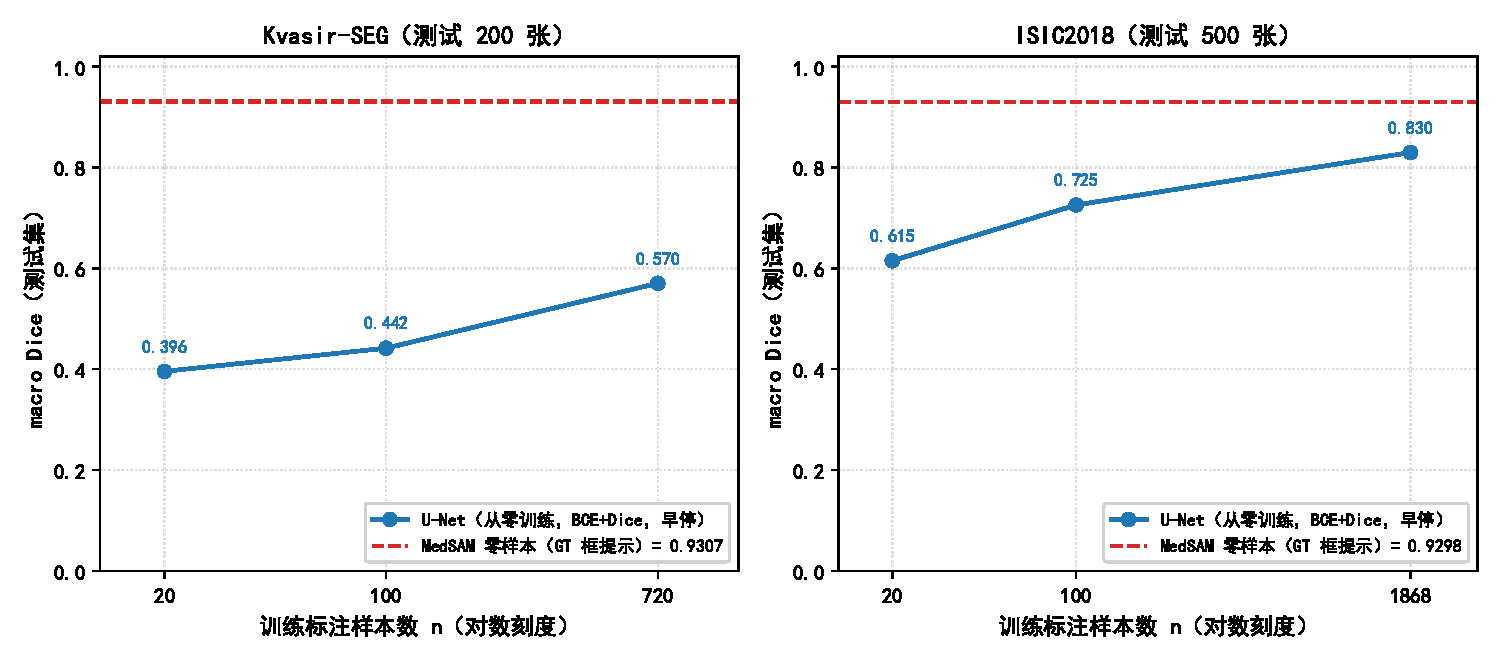
\includegraphics[width=\textwidth]{../figures/learning_curve.pdf}
\caption{实验 B：U-Net 少样本学习曲线（x 轴为标注样本数，对数刻度）。红色虚线为 MedSAM 零样本（GT 框提示）参考线，数值分别为 0.930684（Kvasir-SEG）与 0.929824（ISIC2018），取自与训练实验完全相同的测试集与指标口径。}
\label{fig:curve}
\end{figure}

\begin{table}[htbp]
\centering
\caption{实验 B：U-Net 各标注档位 vs.\ MedSAM 零样本（测试集 macro Dice；``差距'' $=$ MedSAM 零样本 $-$ U-Net）}
\label{tab:fewshot}
\footnotesize
\setlength{\tabcolsep}{4pt}
\begin{tabular}{llrrr}
\toprule
数据集 & MedSAM 零样本（GT 框） & $n=20$ & $n=100$ & $n=$ 全量 \\
\midrule
Kvasir-SEG（全量 $n=720$）  & 0.930684 & 0.395581 & 0.441560 & 0.570244 \\
ISIC2018（全量 $n=1868$）   & 0.929824 & 0.614860 & 0.725499 & 0.829606 \\
\midrule
\multicolumn{2}{l}{差距（Kvasir-SEG）} & 0.535103 & 0.489124 & 0.360440 \\
\multicolumn{2}{l}{差距（ISIC2018）}   & 0.314964 & 0.204325 & 0.100218 \\
\bottomrule
\end{tabular}
\end{table}

两条曲线共同回答了``要多少标注''的问题。\textbf{在统一训练预算内，专用模型即使用尽全部训练标注也未能追平零样本基础模型}：Kvasir-SEG 上 U-Net 从 0.395581（20 张）升至 0.570244（720 张），与 MedSAM 零样本的差距仍达 0.360440；ISIC2018 上 U-Net 从 0.614860 升至 0.829606（1868 张），差距缩至 0.100218。两数据集曲线形态不同：皮肤镜病变（ISIC2018）目标占比大、边界相对清晰，20 张标注即可达 0.61，且随标注量增长平稳上升；内镜息肉（Kvasir-SEG）目标小、对比度低、边界模糊，曲线整体压得更低且更平缓，说明同等标注预算下其学习效率更差。若以曲线外推，ISIC2018 需要数千张量级的标注才有希望进一步逼近 MedSAM 的零样本水平，而 Kvasir-SEG 的差距在当前数据规模下看不到闭合的迹象。这一结果直接刻画了基础模型的价值：\emph{一次框标注（甚至无需像素级掩码）换来的零样本分割质量，超过了数百至近两千张像素级标注训练出的专用模型}。

\subsection{跨数据集泛化}

表~\ref{tab:cross}报告实验 C：将在一个数据集训练池上训练的 U-Net 直接迁移到另一数据集（含跨模态）的测试集，与同域 U-Net（实验 B 全量档位）及 MedSAM 零样本对比。

\begin{table}[htbp]
\centering
\caption{实验 C：跨数据集/跨模态泛化（目标测试集 macro Dice）。同域 U-Net 取实验 B 全量档位；MedSAM 零样本列与实验 A 框提示行为同一测试集上的同一结果（复用，未重推理）。}
\label{tab:cross}
\footnotesize
\setlength{\tabcolsep}{3.5pt}
\begin{tabular}{lrrrr}
\toprule
目标测试集 & U-Net（Kvasir$\rightarrow\cdot$） & U-Net（ISIC$\rightarrow\cdot$） & 同域 U-Net & MedSAM 零样本 \\
\midrule
Kvasir-SEG（$n=200$） & --- & 0.373964 & 0.570244 & 0.930684 \\
ISIC2018（$n=500$）   & 0.238664 & --- & 0.829606 & 0.929824 \\
Montgomery（$n=28$）  & 0.206529 & 0.666025 & ---（未训练） & 0.976842 \\
\bottomrule
\end{tabular}
\end{table}

跨集迁移全面暴露了专用模型``任务绑定''的脆弱性：同域训练的 U-Net 迁移到另一数据集后大幅衰减——ISIC2018 同域 U-Net 达 0.829606，而 Kvasir-SEG 模型迁移到同一目标测试集仅得 0.238664，相对同域水平衰减 0.590942（其中 12 个样本预测为空、按惯例计 0）；Kvasir-SEG 同域 U-Net 为 0.570244，ISIC2018 模型迁移到该目标测试集得 0.373964，衰减 0.196280；跨模态迁移（彩色图像 $\rightarrow$ 灰度胸片）的绝对值更低，Kvasir$\rightarrow$Montgomery 仅 0.206529。与之相对，MedSAM 零样本在全部三个目标模态上保持 0.929824--0.976842，跨模态几乎无衰减。值得注意的是 ISIC$\rightarrow$Montgomery（0.666025）明显好于 Kvasir$\rightarrow$Montgomery（0.206529）：皮肤病变模型习惯分割大块中央暗色区域，与胸片肺野的形态分布更接近；而息肉模型输出的均为小面积圆形掩码，迁移到胸片后几乎完全错位。同域 U-Net 为空缺的 Montgomery 行如实留白——该数据集未训练过 U-Net（其训练集仅 110 张，本文将其保留为跨模态目标域）。该实验为准``基础模型 vs.\ 专用模型''的权衡补上了泛化维度：专用模型的优势被锁死在训练分布之内，而基础模型的零样本能力天然跨分布。

\subsection{定性可视化}

图~\ref{fig:qual}从每个数据集各选 2 个成功与 2 个失败案例（在前 20 张已保存预测的测试样本内，按 MedSAM 框提示与 U-Net 全量档的逐样本 Dice 均值排序选取），对比原始图像、真值掩码与两模型的预测。

\begin{figure}[htbp]
\centering
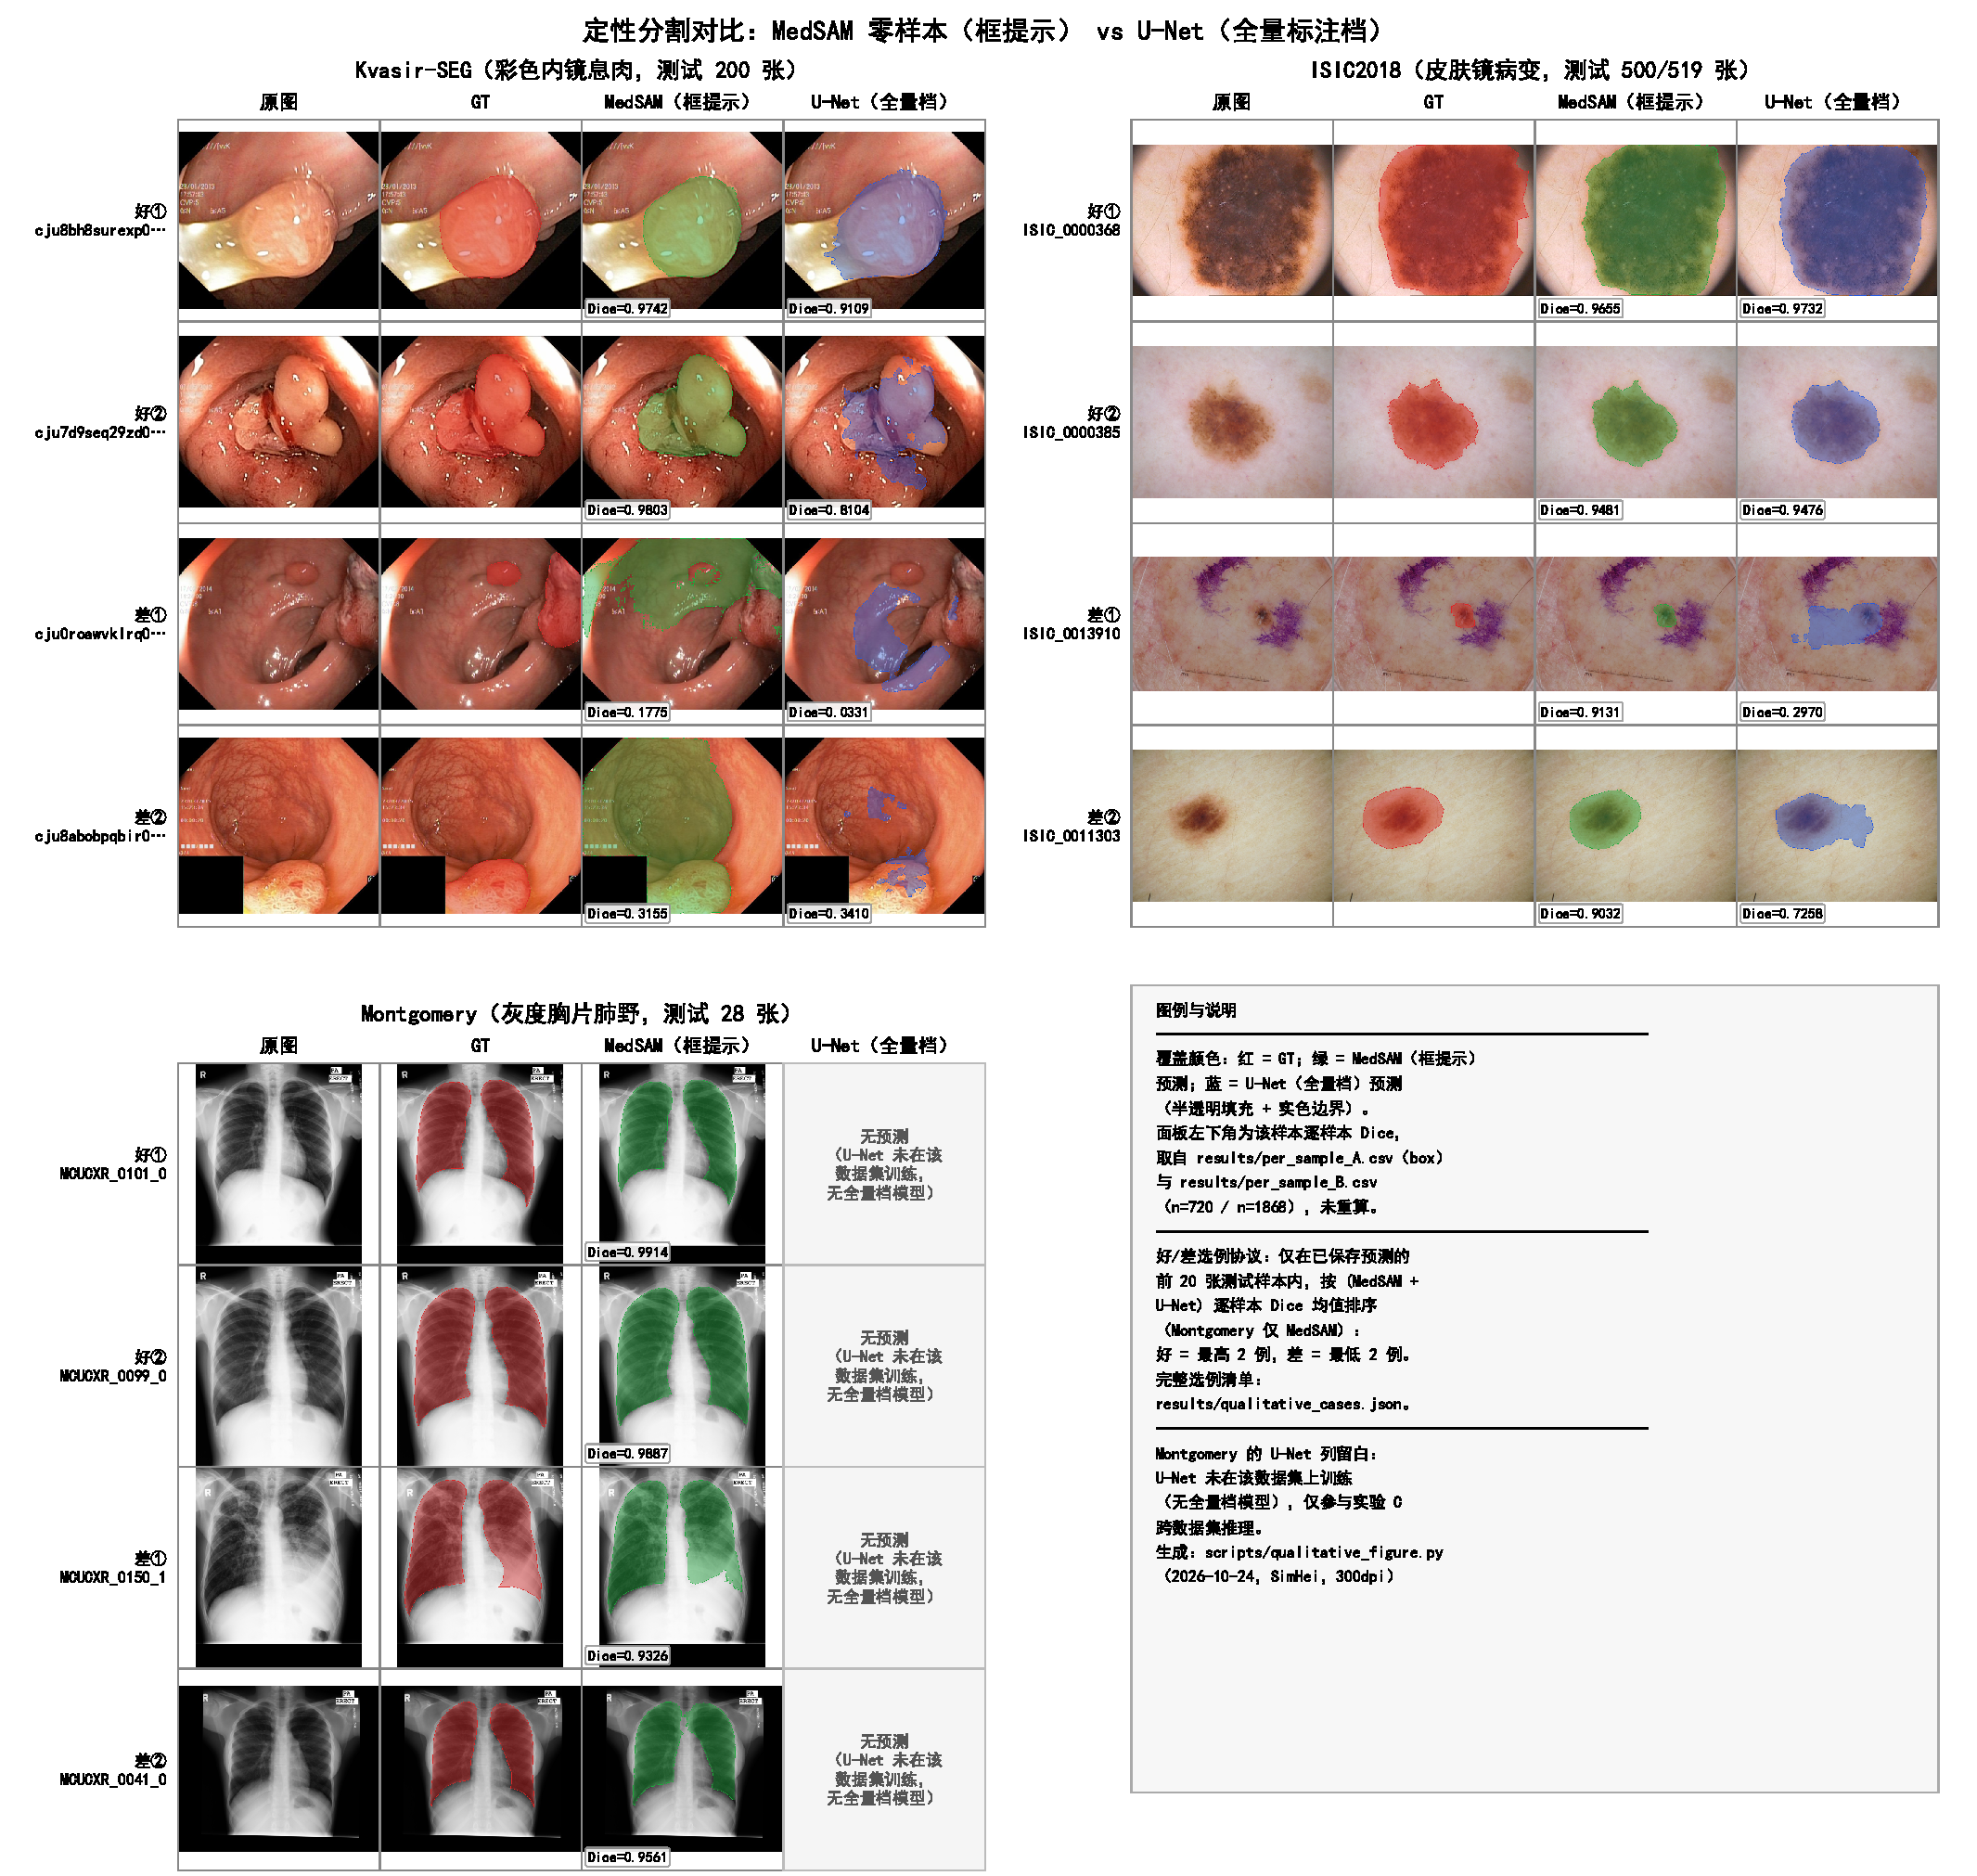
\includegraphics[width=\textwidth]{../figures/qualitative.pdf}
\caption{实验定性对比（每数据集 2 好 + 2 差，按两模型逐样本 Dice 均值排序；绿色为 MedSAM 框提示预测，蓝色为 U-Net 全量档预测，红色为 GT；面板角标为逐样本 Dice）。Montgomery 数据集未训练 U-Net，对应列如实留白。}
\label{fig:qual}
\end{figure}

定性结果与定量表格相互印证。ISIC2018 的失败案例 ISIC\_0013910 展示了基础模型先验的价值：U-Net 全量档在该样本上仅 0.296971（把病灶分割得支离破碎），而 MedSAM 达 0.913090——零样本模型对``医学图像中与框提示匹配的连通区域''有稳定的形状先验，专用模型则可能被训练分布外的表观变化迷惑。Kvasir-SEG 的两个差例（如 cju0roawvklrq079，MedSAM 0.177513 / U-Net 0.033089）则显示两模型会\emph{同时}失败：低对比、边界弥散的息肉对所有方法都构成挑战，这类样本是零样本与少样本方案的共同短板。Montgomery 上即使``差''例的 MedSAM Dice 也在 0.93 以上（最差 0.932585），肺野这类大目标、强先验结构上零样本推理极其稳健。值得注意的是，MedSAM 的失败多伴随掩码整体偏移或欠分割，而 U-Net 的失败更多表现为训练分布外的系统性错位，两者错误模式的差异也与第~\ref{subsec:model}节的协议设定相符。

% ==================== 5 讨论与局限 ====================
\section{讨论与局限}

\textbf{框提示与点提示为何差异巨大。}实验 A 给出 0.93--0.98 与 0.00--0.15 的悬殊对比，其根源在于训练分布：MedSAM 的百万级训练对全部以边界框为提示，模型学到的是``框内找目标''的先验；点提示对其属于分布外输入，伪框实现（固定为图像长边 10\% 的正方形）无法从单个点恢复目标尺度，导致解码器输出与目标严重错位。这提示两点实践准则：其一，部署医学基础模型时应优先采用与训练提示一致的交互形式（框），临床上的框标注（拖一个矩形）成本也远低于像素级勾画；其二，若交互约束只允许点击，应选用原生支持点提示或在混合提示上训练过的模型，而不能依赖框训练模型的``顺便''能力。此外框扰动实验表明，GT 框并非必须精确——$\pm10\%$ 扰动仅损失约 0.05--0.11 Dice，人工粗框已可工作。

\textbf{基础模型与专用模型的权衡。}本文实验描绘了一条清晰的分界线：\emph{在训练分布之内且标注充足时}，专用模型仍有上限优势的可能（本文统一预算下 ISIC2018 U-Net 全量 0.829606 距 MedSAM 零样本仅 0.10，随标注继续增长有望进一步收窄，但不能排除专用模型最终反超）；\emph{在标注稀缺或分布之外时}，基础模型优势是压倒性的——零样本框提示在三个模态上全部高于同预算专用模型，且跨数据集几乎不衰减，而专用模型跨集衰减 $-0.20$ 至 $-0.59$。对临床落地的启示是：新任务起步阶段应以 MedSAM 类模型 + 框提示迅速建立基线，把昂贵的像素级标注预算留给基础模型确实覆盖不了的疑难子集；跨中心、跨设备部署场景下，基础模型的泛化优势尤为关键。

\textbf{局限。}本文结论应在以下边界内理解：（1）\emph{数据规模与模态}——三个数据集覆盖三种模态，但均为公开数据集，Montgomery 测试集仅 28 张，其上所有结论（含跨模态迁移与定性观察）受小样本不确定性影响，只能视为方向性证据；未纳入 CT/MRI 等三维模态。（2）\emph{点提示实现}——点提示经由伪框通路实现（MedSAM 官方推理不支持点），所测得的是``该实现方式下''的下界，原生点提示机制的模型表现可能不同；但这一实现如实反映了 MedSAM 官方代码的实际能力边界。（3）\emph{训练预算}——U-Net 统一 200 epoch 上限、早停与固定超参，这一预算对``少样本能到什么水平''是公平且偏保守的（诊断记录表明 50 epoch 严重欠收敛）；专用模型在更大预算与更精细调参下可能更高，但不改变``全量标注仍未追平零样本''在本文预算下的事实。（4）\emph{指标口径}——macro Dice 逐样本平均，空预测按 0.0 计入（各组合空预测数已如实报告）；未报告 HD95、IoU 等其他指标，边界质量的差异（如 Kvasir-SEG 息肉边缘）可能未充分体现。（5）\emph{框提示依赖 GT}——零样本实验使用真值派生提示，实际部署中框由人工给出，其质量介于本文 GT 框与 $\pm10\%$ 扰动框之间，真实交互下的性能需进一步的人机评估。

% ==================== 6 结论 ====================
\section{结论}

本文以``综述 + 统一协议实验''的方式研究了医学影像分割的基础模型方法。综述部分梳理了从 U-Net 及其变体、nnU-Net 到 SAM、MedSAM 及其医学域适配家族的技术脉络；实验部分在 Kvasir-SEG、ISIC2018 与 Montgomery 三个模态各异的数据集上，以统一的逐样本宏观 Dice 口径得到三个主要发现：其一，MedSAM 零样本推理在 GT 框提示下达到 0.929824--0.976842 的 macro Dice，$\pm10\%$ 框扰动仅损失约 0.05--0.11，而点提示（伪框实现）崩塌至 0.000069--0.148288，提示形式敏感性必须显式验证；其二，统一训练预算下 U-Net 即使用尽全部训练标注（720/1868 张）仍未追平 MedSAM 零样本，差距分别为 0.360440 与 0.100218，且曲线未见闭合迹象；其三，专用模型跨数据集衰减 $-0.196280$ 至 $-0.590942$、跨模态绝对值低至 0.206529，而 MedSAM 零样本跨模态保持 0.93 以上，基础模型的泛化优势得到直接证据支持。综合而言，框提示零样本基础模型已可作为医学分割新任务的默认起点，像素级标注预算应集中投向基础模型失效的疑难样本；后续工作将扩展至三维模态、混合提示训练与参数高效适配，并在人机交互设定下评估真实临床流程中的表现。

% ==================== 参考文献 ====================
\bibliographystyle{plain}
\bibliography{refs}

\end{document}
